\chapter{Экспериментальная часть}

В данном разделе будет произведено сравнение
последовательной реализации трех алгоритмов
и конвейера с использованием многопоточности. А также показана статистика.

\section{Временные характеристики}

Для сравнения возьмем 10 массивов размерностью
$[$5, 10, 25, 50, 100, 250, 1000$]$.
Воспользуемся усреднением массового эксперимента.

Результат сравнения последовательной реализации трех алгоритмов
и конвейера, с использованием многопоточности, представлен на рис. \ref{ref:time}.

\begin{figure}[ht!]
	\centering{
		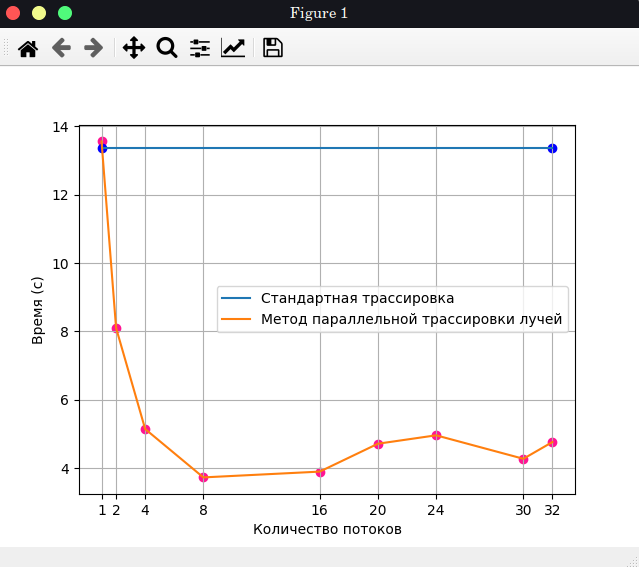
\includegraphics[width=0.8\textwidth]{time.png}
		\caption{Временные характеристики}
		\label{ref:time}}
\end{figure}

По результатам эксперимента видно, что время испольнения конвейерной
реализации значительно меньше, чем исполнение традиционной реализации.
В начале традиционная реализация выигрывает по времени, потому что
при маленьких задачах тратится много времени на создание потоков и
ожидание доступа к переменной, что значительно снижает
работоспособность программы.

На рис. \ref{ref:res} приведена статистика.

\begin{figure}[ht!]
	\centering{
		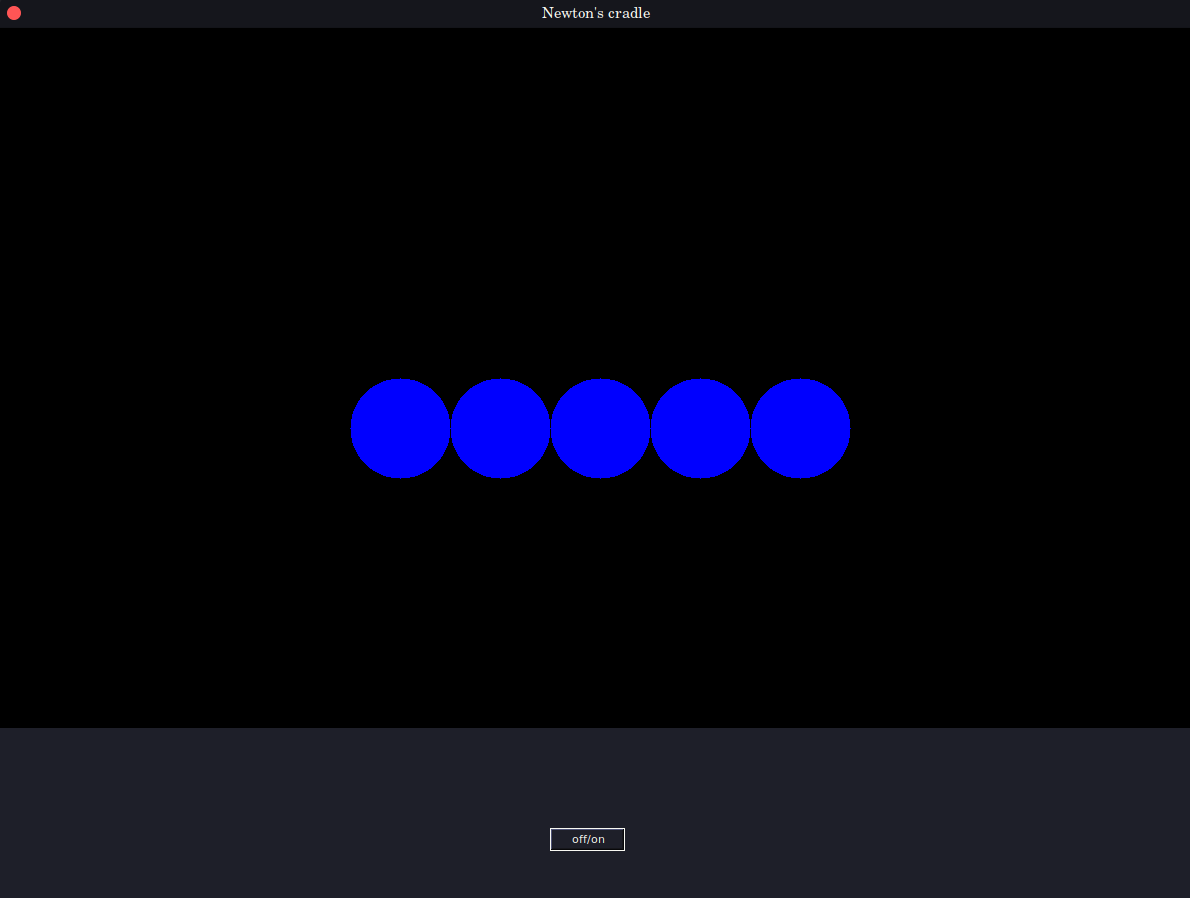
\includegraphics[width=0.6\textwidth]{res.png}
		\caption{Временные характеристики}
		\label{ref:res}}
\end{figure}

\section{Вывод}

В данном разделе было произведено сравнение
последовательной реализации трех алгоритмов
и конвейера с использованием многопоточности.
По результатам исследования конвейерную обработку
нет смысла применять на задачах, занимающих мало времени.
Статистика показала, что конвейерная обработка работает правильно.